% !TeX Options = -shell-escape
\documentclass{panicsoftware-presentation}

\usepackage{tikz}
\usetikzlibrary{decorations.pathreplacing}

\title{What's the lifetime of your object?}
\author{Dawid Pilarski}

\newenvironment{itemizeSeq}{\begin{itemize}[<+-|@alert+>]}{\end{itemize}}
\newenvironment{itemizeNColorSeq}{\begin{itemize}[<+->]}{\end{itemize}}

\begin{document}

\begin{frame}{Agenda}
	\tableofcontents
\end{frame}

\section{What does the title mean?}

\begin{frame}{Title decomposition}

\centerline{What's the \only{lifetime}<1> \only{\alert{lifetime}}<2-> of your \only{object}<1-2> \only{\alert{object}<3>?}}
\pause
\begin{itemizeSeq}
	\item What is a lifetime?
	\item What is an object?
\end{itemizeSeq}

\end{frame}

\begin{frame}{The object}

Objects are:
\begin{itemizeSeq}
	\item created
	\item destroyed
	\item refered to
	\item accessed
	\item manipulated
\end{itemizeSeq}

\end{frame}

\begin{frame}{The Object}

Is created by
\begin{itemizeSeq}
	\item The definition
	\item new expression
	\item when changing active member of a union
	\item creation of the temporary
\end{itemizeSeq}


\end{frame}

\begin{frame}{The object}

Has:
\begin{itemizeSeq}
	\item optional name
	\item storage and it's duration
	\item lifetime
	\item type
\end{itemizeSeq}

\end{frame}

\begin{frame}{The object}

\centerline{Is not a reference {\scriptsize(although reference has lifetime)}}

\end{frame}

\begin{frame}{The variable}

\centerline{Can be either an object or the reference}

\end{frame}

\begin{frame}{Summary: variable, reference, object}
\centering
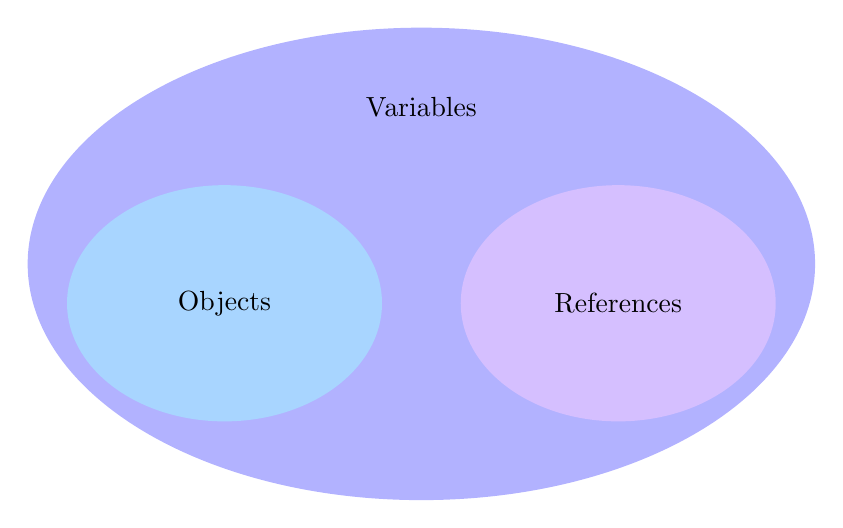
\begin{tikzpicture}
\begin{scope}[blend group=soft light]

\fill[blue!30!white] (0,0) circle[x radius=5cm, y radius=3cm];
\fill[green!60!white] (-2.5,-.5) circle[x radius=2cm, y radius=1.5cm];
\fill[orange!60!white] (2.5,-.5) circle[x radius=2cm, y radius=1.5cm];

\end{scope}

\node at(0,2){Variables};
\node at(2.5,-.5){References};
\node at(-2.5,-.5){Objects};

\end{tikzpicture}

\end{frame}

\begin{frame}{What is lifetime?}

\centerline{Lifetime is a \alert{runtime} property of an object.}

\vfill
\centering

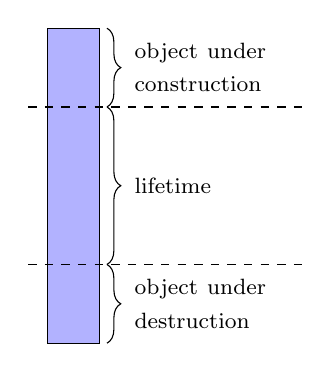
\begin{tikzpicture}

\draw[fill=blue!30!white] (-.75, -2) rectangle (-0.1, 2);

\draw[dashed] (-1, 1) -- (2.5, 1);
\draw[dashed] (-1, -1) -- (2.5, -1);

\draw [decorate, decoration={brace, amplitude=5pt}] (0, 2) -- (0, 1) node[xshift=1.35cm ,midway, text width=2cm]{\footnotesize object under construction};
\draw [decorate, decoration={brace, amplitude=5pt}] (0, 1) -- (0,-1) node[xshift=1.35cm ,midway, text width=2cm]{\footnotesize lifetime};
\draw [decorate, decoration={brace, amplitude=5pt}] (0, -1) -- (0, -2) node[xshift=1.35cm ,midway, text width=2cm]{\footnotesize object under destruction};;

\end{tikzpicture}
\end{frame}

\begin{frame}{What is lifetime?}

\centerline{During the lifetime of an object you can use it without additional restrictions.}

\end{frame}


\begin{frame}{When the lifetime starts}

\centerline{The lifetime of an object starts, when:}

\begin{itemizeSeq}

\item storage with the proper alignment and size for type T is obtained
\item its initialization \alert{(if any)} is complete
\item if the object is a union member or subobject thereof, its lifetime only begins if that union member is the initialized member

\end{itemizeSeq}

\begin{frame}{When you object does not need initialization}




\end{frame}


\end{frame}

\end{document}